\documentclass[8pt]{article}
\usepackage{multicol} % Пакет для работы с колонками
\usepackage{amsmath, amssymb} % Математические пакеты
\usepackage[russian]{babel} % Поддержка русского языка
\usepackage{geometry} % Настройка полей страницы
\usepackage{graphicx}
\usepackage{tikz}
\usepackage{amsmath}
\usepackage{tabularx}
\usepackage{setspace}
\usetikzlibrary{arrows, calc}

\geometry{a4paper, margin=1in}

\begin{document}

\title{}
\author{}
\date{}

\maketitle
\vspace*{-50mm}

\onehalfspacing

\begin{multicols}{2} % Разделение на две колонки

 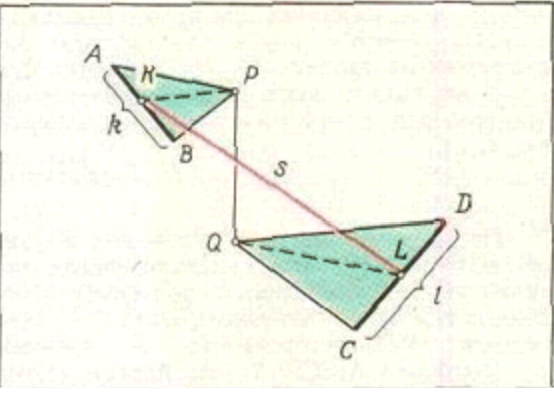
\includegraphics[scale=0.96]{рисунок6.png}

\hspace{-7.5mm} лежат отрезки а и $b$. (В этой и следующих формулах а,  пр$_{a}b $ и т. п. означают длины со-ответствующих отрезков.) Наименьший угол между прямыми не превосходит $ \pi/2,$ поэтому $ cos(a) \ge 0 $ . Из (1) следует равенство 
\newline 
\hspace*{20.0mm} $а$ пр$_{а}b = b$пр$_{b}a,           (2)  $
\newline которое пригодится нам при решении задачи.
\newline
\hspace*{8mm} Обозначим через Р центр верхнего, а через Q - центр нижнего оснований пирамиды. Мы докажем следующий факт, несколько более общий, чем нужное нам утверждение задачи \textbf{M168}.
\newline
\hspace*{8mm} \textit{Пусть плоскости двух подобных равнобедренных треугольников АВР и CDQ С вершинами Р и Q перпендшкилярны отрезку РQ (и, тем самым, параллельны между собой). Обозначим отрезок, совдиклющий середины К и L оснований АВ и СD, через s. Тогда (рис. 6).}
\newline
\hspace*{20.0mm}  пр$_{s}k == l$пр$_{s}l.(3) $
\newline Пользуясь (2), мы вместо (3) можем доказывать такое равенство:
\newline
\hspace*{20.0mm} $ k $ пр ${k}s = l $ пр ${l}s (4). $
\newline Теперь воспользуемся тем, что как это следует из (1), длина пр$b_{a}$ не меняется при параллельном переносе отрезков $a$ и $b$. Поэтому мы можем спроектировать отрезок $k = AB$ на плоскость. треугольника $CDQ$ и получим:
\newline пр$_{A' B'}K'L =$ пр$_{A' B'}KL =$ пр$_{A B}KL =$ пр$_{k}s,$
\hspace*{6mm}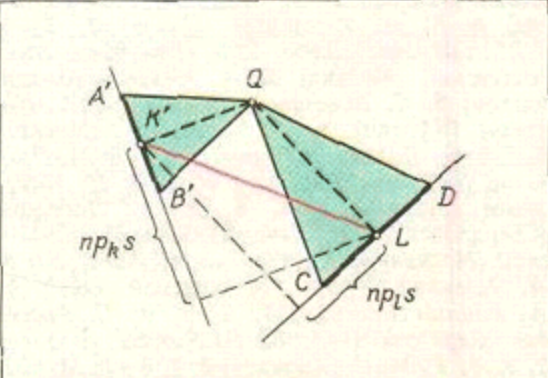
\includegraphics[scale=0.96]{рисунок7.png}
\newline 
где $A', B'$ и $K'$ - проекции точек A, B и K на плоскость $CDQ$(рис.7). Таким образом, мы свели задачу к тому случаю, когда оба треугольника лежат в одной плоскости (и имеют общую вершину). Если отрезки АВ и CD параллельны, то равенство (4) очевидно, поскольку обе проекции равны нулю. Если эти отрезки не. параллельны, то получаем:
 \newline $k/l = {A'B'}/{CD} = {QK'}/{QL} = {sin(QLK')}/{sin(LK'B')}$
\newline 
откуда следует (4).
\newline \textbf{М169}. \textit{Пусть k < n - натуральные числа. Расставьте числа $1, 2, 3, ..., n^{2}$ в таблицу $n \ast n$ так, чтобы в каждой спроке числа в $k$-м столбце а) наименьшей; б) наибольшей.}
\newline
\hspace*{8mm} Решим сначала задачу а).
\newline
\hspace*{8mm} Если расставить числа так, как показано в таблице 1, а - сначала заполнить первые $k$-столбцов, строку за строкой, числами от
PQ (и, тем самым, парали
1 до $kn$, а затем оставшимися числами заполнить последние $(n - k)$ столбцов (как угодно, лишь бы выполнялось условне возрастания чисел в каждой строке)- то сумма 

\scalebox{0.5}{
\renewcommand{\arraystretch}{1.2} % Adjust row spacing
\begin{tabularx}{\linewidth}{c c c c | c | c}
\hline
1 & 2 & ... & k-1 & k & nk + 1... \\ \hline
k+1 & k+2 & ... & 2k-1 & 2k & \\ \hline
2k+1 & 545 & 778 & 7507 & 3k & \\ \hline
... & ... & ... & ... & & \\ \hline
(n-1)k + 1 & 88 & 788 & 6344 & nk & $...n^{2}$ \\[0.5ex]
\hline
\end{tabularx}
}
чисел в $k-$ м столбце будет равна
\newline $k (1 + 2 + ... + n) = \frac{kn(n+1)}{2}.$
\newline Мы докажем, что это значение суммы является наименьшим. Сначала докажем, что если $a_{1}, a_{2}, ..., a_{n} -$ числа $k - $ го столбца, занумерование в порядке возрастания:
\newline 
\hspace*{20.0mm} $a_{1} < a_{2} < ... < a_{i} < ... < a_{n}$
\newline то
\newline 
\hspace*{20.0mm} $a_{i} \ge ki.$
\newline Действительно, рассмотрим числа, стоящие в тех же строках, где стоят ал, ад, ..., ау, н в первых R столбцах. Из условия (2) и условия, что числа в строках стоят в возрастающем порядке, следует, что эти $ki$ чисел не превосходят числа $a_{i}$. Следовательно, среди чисел $1, 2, 3, ..., n^{2}$ имеется по крайней мере $ki$ чисел, не превосходящих $a_{i}$. Отсюда вытекает (3). Сложив неравенства (3) по всем



\end{multicols}

\end{document}